\chapter{Bezvadu Ad Hoc tīkli}\label{sec:infra}
Bezvadu tīklus var sadalīt divās pamatgrupās, tīkli ar iepriekšnoteiktu infrastruktūru un ekspromta tīkli. Tīklu ar iepriekšnoteikto infrastruktūru klasiskais piemērs ir mobilo sakaru tīkls un bezvadu lokālais tīkls (\acs{WLAN}).  Mobilo sakaru tīkla operators izvieto bāzes stacijas tā, lai nodrošinātu bezvadu savienojumu noteiktā diapazonā. Katrai no tīkla bāzes stacijām ir fiksēts ātrgaitas savienojums ar pamattīklu. Datu pārraide bezvadu vidē notiek vienā posmā starp mobilo mezglu un tuvāko bāzes staciju. Bezvadu ekspromta tīkls (\acs{Ad Hoc}) ir decentralizēts bezvadu tīkls \cite{perkinsBook}. Šādu nosaukumu ekspromta tīkls (\acs{Ad Hoc}) ir ieguvis jo tam nav iepriekš noteikta infrastruktūra, no latīņu valodas ''Ad Hoc'' tulkojams kā ''šim nolūkam''.  Ekspromta tīkls pilnībā izslēdz vadu savienojumu no tīkla infrastruktūras. Ekspromta tīkli pielietojami vietās kur tīkla uzbūve ir apgrūtināta vai neiespējama. Dotajā brīdī sensoru tīkli tiek plaši pielietoti militārās operācijās un pētnieciskos projektos kuriem tīkls nepieciešams grūti pieejamos rajonos (piemēram: kalnos, mežos, okeāna dziļumos, u.c.). Kā arī, ekspromta tīklus pielieto iekštelpās, piemēram, konferencēs savienojot vienotā tīklā vairākus klēpjdatorus. Ekspromt tīklā katrs tīklā esošais elements (turpmāk tekstā ''mezgls'') tiek uzskatīts par potenciālo pārraides posmu. Mezgli apvienoti tīklos lai nepieciešamības gadījumā nodrošinātu datu pārraidi. Mezgli varbūt datu avots, saņēmējs vai arī tie var darboties kā retranslējošs mezgls. Ekspromta tīklā mezgli var būt statiski,  mobili vai abi vienreiz. Ad Hoc tīklus var iedalīt sekojošos veidos:
\begin{enumerate}[label=\arabic*)]
    \item \acf{WSN} sastāv no teritoriāli izkliedētiem autonomiem sensoriem kuri novēro fiziskas vai apkārtējas vides izmaiņas, piemēram, temperatūras izmaiņas, vibrācijas, gaisa spiedienu vai piesārņojuma līmeni. Tīklā esošie mezgli izveido savienojumu lai pārraidītu iegūtos datus uz attālinātu pētniecisko centru (\figurename. ~\ref{fig:wsn}). WSN tīkla topoloģija variē no parastas zvaigznes topoloģijas līdz daudzposmu bezvadu režģtīklam (\acs{WMN}) ar tūkstošiem mezglu.
    \item Mobilais ekspromta tīkls (\acs{MANET}) vai Mobilais Ad Hoc tīkls, ir paškonfigurējošs decentralizēts tīkls, kas sastāv no mobilām ierīcēm savienotām savstarpēji ar bezvadu saitēm. Mobilajā ekspromte tīklā (\acs{MANET}) katrā ierīce spēj brīvi pravietoties jebkurā virzienā un nemitīgi mainīt savienojumu partnerus.
    \item Integrēts heterogēnu bezvadu tīkls (\acs{IHWN}) apvieno vienotā tīklā: satelīttīklu, GSM/3G, WiMAX, WPAN, MANET un LAN; aprakstīts IEEE 802.21 standartā.
\end{enumerate}
\begin{figure}[!htb]
\begin{minipage}[t]{0.5\linewidth}
\centering
\includegraphics[scale=0.7]{./graph/wsn}
\caption{Bezvadu sensoru tīkls} \label{fig:wsn}
\end{minipage}%
\begin{minipage}[t]{0.5\linewidth}
\centering
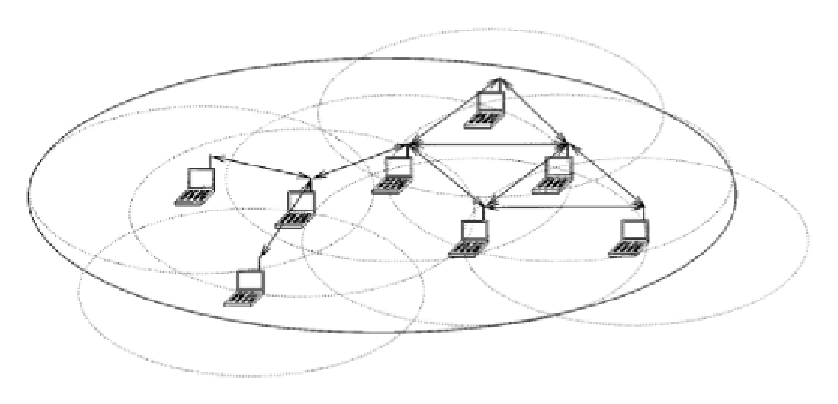
\includegraphics[scale=0.6]{./graph/adhoc}
\caption{Ekspromta tīkls} \label{fig:manet}
\end{minipage}
\end{figure}

\section{WSN un MANET salīdzinājums}
Bieži vien ir grūti noteikt precīzu robežu starp MANET un WSN tīkliem, jo abām topoloģijām ir kopīgas iezīmes un atšķirības ir novērojamas tikai niansēs. Taču šīs nianses izpaužas kā ļoti  svarīgi parametri maršrutēšanas protokolu dizainā.

\subsubsection{Līdzības}
MANET tīkla raksturīpašības ir sekojošas: relatīvi liels mezglu skaits, topoloģija nemitīgi un ātri mainās (dinamiskā topoloģija) un maršrutēšanas protokola pamatuzdevums ir nodrošināt efektīvu datu pārraidi dinamiskos topoloģijas apstākļos. Savukārt, WSN raksturo: ļoti mazas ierīces ar ārkārtīgi ierobežotiem resursiem, koncentrēta mezglu izvietošana, un maršrutēšanas protokola centrālais aspekts ir dati un energoresursu patēriņš. WSN un MANET ir līdzīgi sekojošos aspektos:\\
\small\textbf{\textit{Ad Hoc režīms.}} Nav nepieciešamības iepriekš definēt izmantojamo infrastruktūru vai bāzes staciju (BS). Mezgli savstarpēji sazinās caur vairākām bezvadu saitēm. Katrs tīkla mezgls spēj būt arī avots, galamērķis vai retranslēt paketes.  \\
\small\textbf{\textit{Resursu ierobežojumi.}} Abu tīklu mezgliem ir ierobežoti raidītāja jaudas resursi. Parasti MANET ierīces ir pārnēsājamas ierīces ar zemu raidītāju kapacitāti, piemēram, klēpjdatori, mobilie telefoni, PDA utt.  Sensoriem pieejamie jaudas resursi ir vēl zemāki. \\
\small\textbf{\textit{Enerģijas avotu ierobežojumi.}} Abiem visu mezglu darbība tiek nodrošināta ar mazjaudas akumulatoriem vai baterijām. Viens no svarīgākjiem sistēmas kritērijam ir enerģijas patēriņa samazi- nāšana. Lai ievērojami uzlabot sistēmas veiktspēju ir nepieciešami algoritmi, kas pārrauga enerģijas patēriņu.\\
\small\textbf{\textit{Bezvadu komunikācija.}} MANET un WSN ir izveidoti uz bezvadu komunikācijas kanāla bāzēm.

\subsubsection{Atšķirības}
No pirmā skatiena var rasties iespaids, ka WMN un MANET ir ļoti līdzīgi, taču starp abiem tīkla veidiem ir būtiskas atšķirības.\\
\small\textbf{\textit{Mezglu identificēšana.}} MANET tīklā mezgliem vienmēr ir vispārēji unikāls identifikators (\acs{GUID}), piemēram, MAC adrese vai IP adrese. Tas ir pamat adresēšanas princips visiem MANET maršrutēšanas protokoliem. WSN tīklā GUID tiek pielietots pēc nepieciešamības (ar AODV vai OLSR protokoliem) un iespējām.\\
\small\textbf{\textit{Resursi.}} Abiem - MANET un WSN tīkliem ir ierobežoti resursi, bet kritiskais līmenis katram ir savs. MANET mezglu resursi ir daudzkārt augstāki nekā WSN. MANET tīkls pārsvarā sastāv no pārnēsājamām ierīcēm, kuru procesora kapacitāte sasniedz simtus MHz; iebūvētās atmiņas tilpums ir no dažiem megabaitiem līdz gigabaitiem, to var palielināt ar atmiņas kartēm; akumulatoru kapacitāte nodrošina ierīces vairāku stundu darbību. Savukārt, WSN sastāv no ierīcēm ar ārkārtīgi ierobežotiem resursiem. Piemēram, Berkeley MICA2 sensors ir aprīkots ar 8-bitu ATmegall128 procesoru, iebūvētu 128K RAM, 4K EEPROM un 512K atmiņas karti \cite{Proc13}.\\
\small\textbf{\textit{Komunikācijas paradigma.}} MANET tīklā visi mezgli ir vienranga (peer-to-peer). Nevienam mezglam nav prioritātes un datu pārraidi var iniciēt ikviens tīkla mezgls. Apraide (broadcast) izmantota tikai maršruta izveidošanas procesā (handshake apmaiņai), savukārt ziņojumu pārsūtīšanai izmanto GUIDS adresi un ziņojumi adresēti vienam noteiktam galamērķim. WSN tīkla galveno lomu aizņem satekne (sink), tā ir vienīgā vārteja (gateway) starp tīklu un galalietotāju (\figurename. ~\ref{fig:wsn}). Satekne vienmēr iniciē datu pārraidi tīklā. Mezglu savstarpēja komunikācija ir reta parādība bezvadu sensoru tīklā. Savukārt, apraide un multiraide (multicast) ir ļoti bieži sastopama WSN tīklos, to ietekmi vienmēr jāņem vērā.\\
\small\textbf{\textit{Blīvums.}} Mezglu blīvums $\rho$ tiek definēts kā vidējais kaimiņ-mezglu skaits uz vienu mezglu tīklā \cite{NSsurvey}. Izmantojot disku grafu komunikācijas modeli (Unit Disk Communication Model) to aprēķinā pēc formulas \cite{perkinsBook}
\begin{equation}
\rho=\frac{(N\pi r_{link}^2)}{A} ,
\label{eq:blivums}
\end{equation}
kur $N$ ir kopējais sensoru skaits tīklā, A ir tīkla laukums un $r_{link}$ ir mezgla radio pārraides diapazons. MANET tīklos mezgli ir reti izkliedēti tīkla laukumā, turpretim WSN mezglu izvietojums ir biezs. Dažādu blīvumu dēļ tiek izmantoti dažādi paņēmieni robustuma novēršanai. Piemēram, MANET protokolā datu posms nodrošina lēkumu pārraidi un šī savienojuma izturība ir ļoti svarīga. Maršrutēšanas protokolu dizainā pievērš lielu uzmanību savienojuma izveidošanai un tā ilgstošai pastāvēšanai. WSN tīklos datu pārraide notiek bez apliecinājumu (acknowledgment) mehānisma pielietošanas, jo vienaposmā (one-hop) savienojums var būt ļoti nedrošs. No iepriekš minētā var secināt, ka pārraides kanāla noturība ir ļoti svarīgs aspekts \cite{20}.\\
\small\textbf{\textit{Bezvadu multiraides priekšrocība.}} WSN tīkla mezgls multiraides režīmā spēj vienlaicīgi raidīt datus $r_{link}$ diapazonā esošajiem kaimiņiem. Līdz mezgliem, kas atrodas ārpus šī diapazona, ziņojums nonāks kā troksnis. Savukārt, MANET tīklā pārraide notiek uz vienu noteiktu adresi.  \\
\small\textbf{\textit{Dizaina kritēriji.}} MANET tīklu galvenie izveidošanas un vērtēšanās kritēriji ir servisa kvalitāte (\acs{QoS}) un kanāla caurlaidspēja. Enerģijas patēriņš tiek atvirzīts otrajā plānā, jo ierīces akumulators var tikt nekavējoties uzlādēts vai aizvietots. WSN tīkls sastāv no liela neaprūpēta ierīču skaita, kurā akumulatora aizvietošana vai uzlādēšana ir sarežģīts proces. Līdz ar to maršrutēšanas galvenais mērķis ir pazemināt enerģijas patēriņu lai pagarinātu tīkla darbības laiku.\\
\small\textbf{\textit{Protokolu dizains.}} MANET tīkla protokoli tiek izveidoti pēc slāņu koncepcijas, kas savukārt ir iemantota no vadu tīkliem. Turpretī, WSN tīkls ir izveidots uz iegultās sistēmas (embedded system) bāzes un šai gadījumā ''visi-vienā'' (all-in-one) dizains ir piemērotāks. \\

\section{WSN un WMN salīdzinājums}
Bezvadu režģtīkls (WMN) sastāv no mezgliem kas caur bezvadu savienojumu retranslē citu mezglu paketes (\seename ~\figurename.~\ref{fig:wmn}, ar punktēto līniju apzīmēts bezvadu savienojums).
\begin{figure}[!htb]
\centering
\includegraphics[scale=1]{./graph/wmn}
\caption{Bezvadu režģtīkls \cite{perkinsBook}}
\label{fig:wmn}
\end{figure}

 WMN tīklu pamatuzdevums ir retranslēt paketes  līdz režģtīkla globālā tīmekļa vārtejām (\figurename.~\ref{fig:wmn} ''Internet gateway''). Parasti režģtīkla mezglam ir raksturīgi sekojoši parametri: mezgli stacionāri, vai arī tiem piemīt minimāla mobilitāte; mezgli ir izvietoti uz māju jumtiem vai ielas apgaismojuma stabiem; atsevišķas vārtejas ar vadu ir savienotas ar pamattīklu. Mezgli aprīkoti ar vairākiem interfeisiem: Wi-Fi, Ethernet, Bluetooth un citi.

Kā pāradīts \figurename.~\ref{fig:wmn} WMN perfekti der pilsēttīkla (\acs{MAN}) izveidošanai. WMN spēj nodrošināt augstāku datu pārsūtīšanas ātrumu nekā mobilo telefonu tīkls, līdz ar to var nodrošināt kvalitatīvu IP balss pārraidi (VoIP) un citus multimediju servisus.
Pēc savas koncepcijas WMN it līdzīgs MANET, tas ir tādā ziņā, ka mobilās stacijas savā starpā komunicē izmantojot daudzposmu pārraidi. MANET un WMN ir būtiskas atšķirības:
\begin{itemize}
\item Režģtīkla mezgli pārsvarā ir stacionāri un tas ietekmē protokolu dizainu, savukārt MANET mezgli ir mobili.
\item WMN tīkla caurlaidspēja ir svarīgs faktors, jo WMN tīklā spēj operēt simti vai pat tūkstoši mezglu. Arī tīkla mērogojamība ir svarīgs jautājums WMN tīkla dizainā.
\item Enerģijas patēriņš nav tik svarīgs, jo pamatā režģtīkla mezgli ir tieši savienoti ar elektroenerģijas tīklu. Tas ļauj izmantot jaudīgāku aparatūru režģtīkla mezgliem.
\end{itemize}

\section{Bezvadu interfeiss}
Ad hoc tīklos ir pielietojamas vides piekļuves vadības (\acs{MAC}) balstītas bezvadu tehnoloģijas, kas pārsvarā darbojas ISM frekvenču joslā (Industrial Scientific and Medical band). Radio kanāli, kas darbojas ISM frekvences joslā, saņem papildus interferenci no tīklā neiesaistītām ierīcēm kas darbojas ISM, piemēram, mikroviļņu krāsnis. Šajā sadaļā netiks apskatīti visi IEEE 802 ģimenes standarti, bet tikai tie ar kuriem aprīkots vairākums no PDA, portatīvajiem datoriem kā arī mobilie telefoni un kurus iespējams izmantot Ad Hoc tīklu izveidē.

\begin{table}[!ht]
    \begin{tabular}{|l|c|c|c|c|c|c|}
        \hline
~              &802.11a&802.11b&802.11g&802.11n&802.15.1&802.15.4\\ \hline
Frekvence,[GHz]&5      &2.4    &2.4    &2.4    &2.4,     &2.4\\
              ~&      ~&      ~&      ~&     ~ &5        &0.868,0.915\\
Tehnoloģijas   &OFMD   &DSSS   &OFMD   &OFDM   &FHSS     &DSSS\\
Pārraid.ātrums,[Mbit/s]&54     &11     &54     &250      &3  &20-250$^{1}$\\
Antenas jauda,[mW]&20-40&100   &20-50  &250    &1,2.5&1\\
Diapazons,[m]  &120     &140   &140    &250    &10       &75\\
Tips           &\multicolumn{4}{c|}{WLAN}&\multicolumn{2}{c|}{WPAN}\\
 Enerģ.pateriņš Tx [mA]&\multicolumn{4}{c|}{400+}&40     &30\\
      'standby' režīma [mA]  &\multicolumn{4}{c|}{20}&0.2        &3\\\hline
\multicolumn{7}{r}{ \footnotemark[1]\footnotesize{Kbit/s}}
    \end{tabular}
\caption{IEEE 802 standartu apkopojums}
\end{table}

\begin{figure}[!htb]
 \centering
\includegraphics[scale=0.6]{./graph/wireless.png}
\caption{IEEE 802 bezvadu tehnoloģijas}
\end{figure}

% B. Mac Protocol - IEEE 802.11 Standard
% The distributed coordination function (DCF) of IEEE 802.11 [10] for wireless local area networks (WLANs) is used as the medium access control (MAC) protocol. The IEEE 802.11 DCF uses Request-to-send (RTS) and Clear-to-send (CTS) control packets for “unicast” data transmission to a neighboring node. The RTS/CTS exchange anticipates the data packet transmission and implements a form of virtual carrier sensing and channel reservation to reduce the impact of the well-known hidden terminal problem [11]. Data packet transmission is followed by an acknowledgment (ACK). All the packets are transmitted at maximum power. “Broadcast” data packets and RTS control packets are sent using physical carrier sensing. An un-slotted CSMA technique with collision avoidance (CSMA/CA) is used to transmit these packets. The considered node model has characteristics similar to those typical of the commercial radio interface in Lucent’s WaveLAN [12].



\subsection{IEEE 802.11}
Šobrīd visplašāk  pieejamais bezvadu datu pārraides interfeiss ir IEEE 802.11 ģimenes tehnoloģijas, kas pārsvarā darbojas 2.4 GHz frekvenču diapazonā izņemot IEEE 802.11a 5 GHz. Wi-Fi datu pārraides segums ir atkarīgs no  ierīces antenas jaudas un vides kurā signāls izplatās. Tīkla pārklājums variē no 50 līdz 100 metriem.

\subsubsection{IEEE 802.11a}
IEEE 802.11a izmanto ortogonālo frekvenčdales multipleksēšanas (\acs{OFDM}) tehnoloģiju un ir vienīgā bezvadu radio tehnoloģija kura darbojas 5 GHz frekvenču joslā.  IEEE 802.11a standarta datu pārraides ātrumi varbūt [6, 9, 12, 18, 24, 36, 48, 54] Mbit/s. Standartā rekomendējamais datu pārraides ātrums ir 24 Mbit/s, bet IEEE802.11a ierīču ražotāji palielina to līdz 54 Mbit/s (tas ir atļauts standartā). 54 Mbit/s ir maksimālais pārraides ātrums, bet reālistiskos apstākļos sasniedz 24 Mbit/s. Pēc CISCO publicētiem datiem pārraides jauda ir 40 mW pie [6 - 24] Mbit/s un 20 mW pie maksimāla datu pārraides ātruma 54 Mbit/s \cite{cisco}.

\subsubsection{IEEE 802.11b}
IEEE 802.11b izmanto tiešās secības spektra paplašināšanas (\acs{DSSS}) tehnoloģiju un darbojas 2.4GHz frekvenču joslā. Datu pārraides ātrums ir [1, 2, 5.5, 11] Mbit/s. Datu pārraides distance ir 90 m pie 1 Mbit/s un ap 30 m pie 11 Mbit/s. Ar maksimālo jaudu 100 mW pie visiem pārraides ātrumiem \cite{cisco}. No IEEE 802.11 ģimenes standartiem šis standarts ir viss biežāk pieejams mobilajās ierīcēs.

\subsubsection{IEEE 802.11g}
IEEE 802.11g tāpat ka IEEE 802.11a izmanto izmanto OFDM, un kā IEEE 802.11b darbojas 2.4GHz frekvenču joslā. Maksimālais datu pārraides ātrums ir 54 Mbit/s, savukārt reālistisks ir 22 Mbit/s. Tapat kā IEEE 802.11a standartā datu pārraides ātrums var būt [6, 9, 12, 18, 24, 36, 48, 54] Mbit/s un antenas pārraides jauda ir 50 mW pie [6 - 24] Mbit/s un 20 mW pie 54 Mbit/s \cite{cisco}.

\subsection{IEEE 802.15}
IEEE 802.15 standarts nosaka bezvadu personālā apgabala tīkla (\acs{WPAN}) standartus. Tas iekļauj informāciju par fiziskā (PHY) un \acs{MAC} slāņa specifikāciju bezvadu savienojumiem izveidošanai stacionārām, portatīvām un mobilām ierīcēm, kas darbojas PAN apgabalā.

\subsubsection{IEEE 802.15.1}
IEEE 802.15.1 standartā aprakstītā tehnoloģija ir plašāk pazīstama kā Bluetooth tehnoloģija. Bluetooth signāla modulācijai izmanto frekvences lēkāšanas (\acs{FHSS}) tehnoloģiju, kas arī darbojas 2.4 GHz frekvenču joslā. Šīs tehnoloģijas datu pārraides diapazons ir ierobežots līdz 10 metriem un datu pārraides ātrums ir 1 Mbit/s. Bluetooth antenas jaudas: Klase 1 ir 100 mW ar raidīšanas distanci $\approx$ 100m; Klase 2 ir 2.5 mW ar distanci $\approx$ 10 m; Klase 3 ir 1 mW ar distanci $\approx$ 5 m.

\subsubsection{IEEE 802.15.4/ZigBee}
IEEE 802.15.4/ZigBee tehnoloģija izmanto tiešās secības spektra paplašināšanas (\acs{DSSS}) tehnoloģiju un darbojas 2.4 GHz, 915 MHz un 868 MHz frekvenču joslās. Datu pārraides ātrums ir 250 Kbit/s pie 2.4 GHz, 40 Kbit/s pie 915 MHz un 20 Kbit/s pie 868 MHz. IEEE 802.15.4 MAC slānis ir nesēja jušanas un sadursmju nepieļaušanas daudzpiekļuves (\acs{CSMA/CA}) metodi, tapāt kā IEEE 802.11 ģimenes standarti. Datu pārraides diapazons ir no 10 līdz 75 metriem un antenas jauda ir 1 mW.
Šeit svarīgi atzīmēt ka ZigBee nav IEEE 802.15.4 standarts. IEEE 802.15.4 standarts ir zemo-ātrumu bezvadu personālā apgabala tīkls (\acs{LR-WPAN}), savukārt ZigBee ir specifikācija kurā PHY un MAC slāņos izmanto IEEE 802.15.4 standartu.
\begin{figure}
\centering
\includegraphics[scale=0.95]{./graph/zigBee.png}
\caption{IEEE 802.15.4/Zigbee \cite{libelium}}
\end{figure}

% \section{Tehnoloģijas izvēles pamatojums}
% WSN tīklu galvenas raksturīpašības ir: augsts mezglu blīvums, ierobežots enerģijas avots, Ad-Hoc režīms. No IEEE 802 standartu ģimenes IEEE 802.15.4/ZigBee standarts izpilda visas. Pirmkārt ZigBee nodrošina zemo enerģijas patēriņu ar to ka tam ir tikai divi darbības režīmi: 1)Pārraides/Uztverēs un 2)miega (Sleep). Atkarība no ierīces konfigurācijas (galvenokārt raidītajā jaudas)  baterijas darbības laiks variē no mēnešiem līdz pat gadiem. Otrkārt, ZigBee ierīces spēj darboties trijās ISM joslas: 2.4GHz un 868/915 MHz. Augstfrekvences josla ir vispasaules pieejama un zemāka josla Ziemeļamerikā, Eiropā, Austrālijā un Jaunzēlandē. Un treškārt ZigBee varbūt dažādas topoloģijas: zvaigžņtīkla, režģtīkla un  vienādranga arhitektūra.
% \begin{table}[!ht]
%     \begin{tabular}{|c|l|l|l|}
%         \hline
% Frek. josla,[MHz]& 868.3&902-928&2400-2483.5\\ \hline
% Kanālu sk.&1&10&16\\
% Joslas platums,[KHz]&600&2000&5000\\
% Pārraides ātrums,[Kbit/s]&20&40&250\\
% Symbol Rate[1/sec]&20&40&62.5\\
% Frek. stabilitāte&\multicolumn{3}{|c|}{40ppm}\\
%         \hline
%     \end{tabular}
% \caption{IEEE 802.15.4 standarta PHY slāņa parametri}
% \end{table}